\chapter{Estudio de Reuseport}

Como ya se estudió, los problemas del escenario multihilo reconocidos en los capítulos anteriores impactan principalmente en los tiempos de lectura de interfaces de red, donde bajos tiempos son siempre un elemento prioritario a garantizar. Entendiendo éste problema es que varios gigantes de la industria han planteado mecanismos alternativos que permitan aprovechar mejor los recursos de los computadores de arquitecturas modernas al emplear programación paralela. En ésta linea, la propuesta más prometedora hasta la fecha es la brindada por Google, denominada \emph{Reuseport}.

Reuseport \cite{slides:googleReuseport} es una de las soluciones más usadas para hacer frente al problema descrito, por su gran efectividad en la practica. Corresponde a un desarrollo de Tom Herbert --Ingeniero de Google-- desarrollado precisamente para responder a los bajos desempeños generados al emplear un esquema de consumo de sockets como el planteado hasta el momento. El trabajo de Herbert plantea que las distintas estratégias que se puedan adoptar sobre un único socket para mejorar la performance en su acceso concurrente terminan no resultando efectivas por mantener el punto de contención al compartir la misma estructura, lo que vendría siendo el origen del problema y se presenta disponible (según el mismo autor) desde la versión 3.9 del kernel de Linux\footnote{En la actualidad, la característica reuseport ha sido portada a otras versiones del kernel, estando disponible en versiones desde la 2.6 en variadas distribuciones de Linux.}.

\begin{figure}[h!]
	\centering
	\hspace*{\fill}
	\subfigure[Puerto tomado por un socket tradicional.]{
		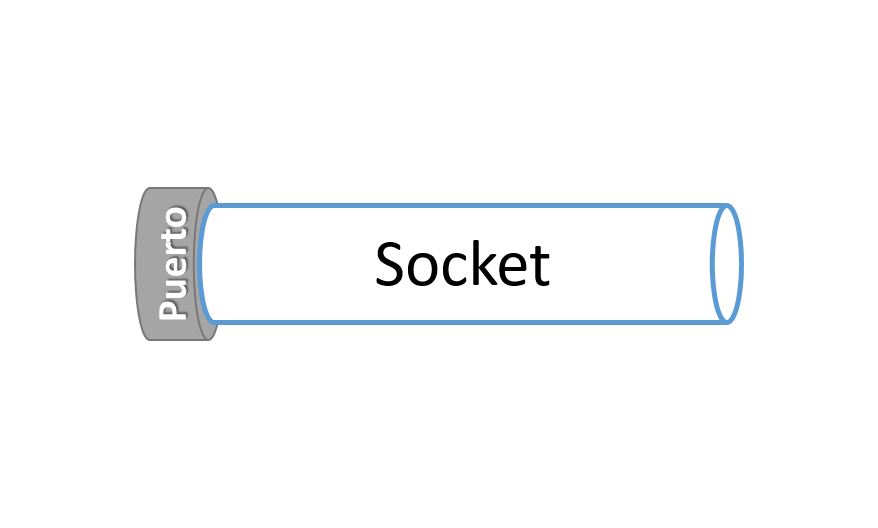
\includegraphics[width=.45\textwidth]{imagenes/socketNormal.png}
	}\hfill
	\subfigure[Compartición de puerto usando reuseport.]{
		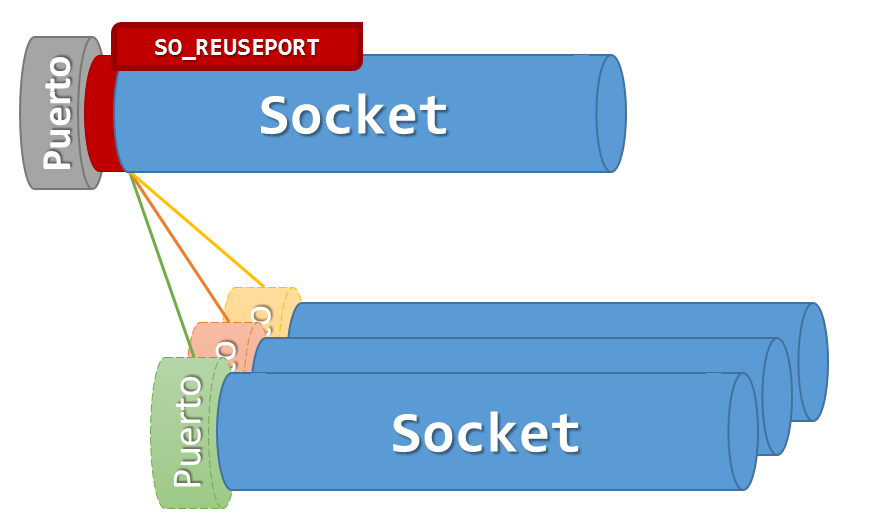
\includegraphics[width=.45\textwidth]{imagenes/socketReuseport.png}
		\label{fig:soReuseport}
	}
	\caption{Comparativo del funcionamiento de asociación sockets-puerto usando sockets tradicionales con respecto a sockets con la opción reuseport.}
	\label{fig:socketHandshake}
	\hspace*{\fill}
\end{figure}

Reuseport se plantea como una opción para los sockets estándar de Linux que promete una mejora en los tiempos de consumo en la atención a un determinado puerto. Dicha opción permite compartir un mismo puerto local del sistema entre múltiples sockets distintos. De ésta manera, conservando el esquema multithread, cada thread puede tener exclusividad en el consumo de un socket eliminando el punto de contención único que se ocaciona al compartir un único socket. Al usar la opción reuseport la tarea de distribución de paquetes entre los distintos sockets que compartan un puerto local es delegada directamente al kernel, el cual asigna aleatoreamente los paquetes recibidos entre los sockets que escuchan el mismo puerto.

\section{Implementación}
La opción está implementada íntegramente en el código fuente del kernel, distribuida entre distintos archivos que hacen uso de la misma. Por sólo mencionar algunos, los archivos responsables de los mecanímsos de conexión en capa IP\footnote{\url{http://lxr.free-electrons.com/source/net/ipv6/inet6_connection_sock.c?v=3.14}}, la implementación de los sistemas de tablas de hash para el módulo de red\footnote{\url{http://lxr.free-electrons.com/source/net/ipv6/inet6_hashtables.c}}, los mecanísmos base de la api de conexiones de los sockets de internet\footnote{\url{http://lxr.free-electrons.com/source/net/ipv4/inet_connection_sock.c?v=3.18}} y la mismísima implementación de UDP en el kernel\footnote{\url{http://lxr.free-electrons.com/source/net/ipv4/udp.c}} se han visto tocadas.

La opción está diseñada para habilitarse por medio de la llamda a sistema \verb=setsockopt()= indicando el descriptor del socket a habilitar y especificando como identificador para ésta opción el flag \verb=SO_REUSEPORT=, que es una constante incluída de los encabezados de \verb=socket.h= del kernel mismo. El socket sobre el que se habilite la opción debe ser el primero en tomar posesión del puerto en cuestión para poder compartirlo con otros sockets (ya sea que estos últimos cuenten con la funcionalidad reuseport habilitada o no).

El mecanísmo de distribución de paquetes que emplea el kernel se basa en una tabla de hash que aprovecha una 4-tupla de valores correspondientes a los mismos valores de las tuplas de direccionamiento constitutivas de un paquete según el modelo OSI. En la práctica, reuseport dispone de un mecanímso de hash que usa los identificadores de ip y puerto (de origen y destino en ambos casos) para la construcción del registro en la tabla de hash. La función de distribución del hash está confeccionada para lograr una distribución uniforme de valores \cite{article:reuseport}.


\section{Uso en la práctica}
Como se mencionó, para usar ésta opción se debe modificar la estructura socket que primero tome control del puerto local para escucharlo por medio de la llamada \verb=bind()=. Con ello, el puerto puede ser posteriormente re-acoplado por otros sockets sin la necesidad de que éstos últimos tengan la característica activada (Ver imagen \ref{fig:soReuseport}).

La adopción de ésta funcionalidad ha sido incorporada a distinto software con requerimientos común de alta disponibilidad de atención de consultas con buenos resultados. Ejemplos de lo anterior son productos como \emph{nginx}\footnote{\url{https://www.nginx.com/blog/socket-sharding-nginx-release-1-9-1/}} o \emph{Apache Web Server} \cite{paper:apache} que han incorporado ésta característica en versiones recientes con buenos resultados.

\section{Rendimiento en la Práctica}
Para evaluar el rendimiento práctico de la opción reuseport se modificó sutilmente el caso de estudio evaluado a lo largo de la investigación para hacerlo compatible con éste enfoque de trabajo. Recordémos que reuseport se basa en la acción de múltiples sockets consumiendo datos, ya no sólo uno, por lo que hay ciertas salvedades que estipular. Al igual que en el escenario original, el objetivo es calcular el tiempo de consumo de 1 millón de paquetes desde un socket UDP en escenario de saturación. La diferencia en éste caso radica en que, en pos de aprovechar las promesas de reuseport, se cambia el consumo concurrente desde el mismo socket usando múltiples hilos por un consumo de múltiple hilos que consume cada uno a un socket distinto, alocado en la misma interzaf lógica del sistema del socket saturado usando la opción reuseport. De ésta manera, el consumo por socket ahora es exclusivo para cada thread, eliminando el punto de contención detectado en la prueba original.

\begin{figure}[!h]
	\centering
	
\includegraphics[scale=.3]{imagenes/fcfm}
	\caption{Nuevo esquema de la prueba UDP en escenarios donde se aproveche Reuseport.}
	\label{fig:casoPruebaReuseport}
\end{figure}

Para poder llevar a cabo ésta prueba, y siguiendo el régimen de operación que exige ésta solución, es necesario garantizar que el primer socket creado para la recepción de datos posea la opción \verb=SO_REUSEPORT= habilitada. Además la cantidad total de consumo (1 millón de paquetes) debe ser redistribuida entre los sockets que se evalúen. La medición de tiempos en éste caso debe ser en función del último socket que termine el consumo de su cuota, pues dicho tiempo representa el tiempo total en que se completa la transferencia total en relación al caso de estudio original. A modo de formalización, se estipúlan los siguientes conceptos importantes en el nuevo caso de estudio:
\begin{description}
\item[Tiempo Mínimo] Corresponde al tiempo en que el primer socket termina de consumir su cuota de consumo asignada.
\item[Tiempo Neto] Corresponde al tiempo en que el último socket termina de consumir su cuota de consumo asignada. De esta forma, corresponde al tiempo en que se completa la trasferencia total de datos.
\item[Cuota de Consumo] Corresponde a la porción de paquetes que le corresponde consumir a cada socket. Si el envío total se denomina como $N$ y se tienen $k$ sockets para emplear el consumo con reuseport, la cuota de consumo de cada uno es el cociente $\frac{N}{k}$. El valor de la cuota de consumo es una restricción de diseño que impone la implementación de reuseport al usar un hash de distribución uniforme, por lo que en éste caso, el valor es idéntico para cada instancia socket.
\end{description}

Un esquemático de ésta prueba puede apreciarse en la figura \ref{fig:casoPruebaReuseport}. La figura \ref{fig:resultadosReuseport} ilustra los tiempos obtenidos a lo largo del nuevo caso de estudio. Sorprendentemente, reuseport consigue tiempos netos gradualmente mejores a medida que se incorporan threads hasta un tope en torno a los 8 sockets donde el rendimiento se estanca para luego empeorar. Otro aspecto interesante es una característica no documentada, y es que según los resultados obtenidos, reuseport garantiza un tiempo de operación mínimo basado sólo en el consumo por socket. Vale decir, el tiempo en que el primer socket completa su cuota (tiempo minimo) está relacionado a ser directamente proporcional a la cuota de consumo. Luego, como a medida que se incorporan más y más sockets la cuota de consumo se reduce (en medida exponencial en nuestro experimento), y así también el tiempo mínimo se reduce de la misma manera.

\begin{figure}[!h]
	\centering
	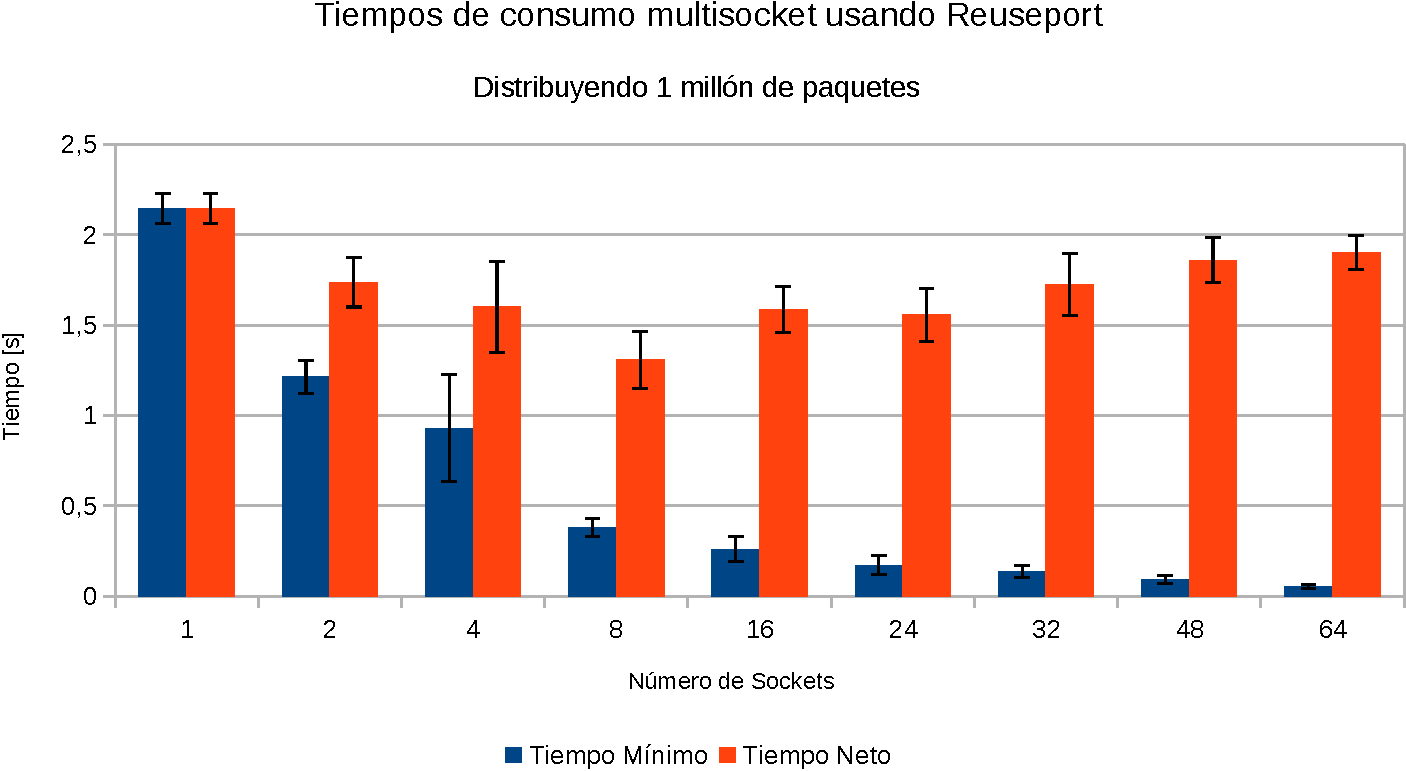
\includegraphics[scale=.6]{resultados/reuseport1-crop.pdf}
	\caption{Gráfico con tiempos de consumo de reuseport para el nuevo caso de estudio.}
	\label{fig:resultadosReuseport}
\end{figure}

\subsection{Diferencias entre arquitecturas}
[[[[[[Aun pendiente sobre si va esto]]]]]]]]]

\section{Evaluación de Optimizaciones Adicionales}
Los resultados anteriores evidencian un claro incremento en el rendimiento alcanzable por la prueba ya conocida aprovechando múltiples sockets en el consumo. Sin embargo cabe preguntarse si será posible mejorar aún más esos resultados combinando la opción de reuseport con técnicas de consumo concurrente sobre los sockets. Una hipótesis que apoya ésta idea se basa en que, al emplear la opción reuseport, los sockets tienen una menor cuota de consumo cada uno, por lo tanto, un acceso concurrente en ese escenario de bajo consumo podría impactar en una reducción de tiempos finales al generar una nula sobrecarga en cada caso.

\subsection{Incorporación de Multithreading}
En la presente sección se validará el rendimiento alcanzable por la opción reuseport usándola en combinación con diferentes estratégias de multithreading como las vistas en el capítulo anterior. Para éste caso, se evaluó el mismo caso de estudio anterior considerando además distintas configuraciones de consumo concurrente para cada instancia de socket, probando configuraciones con 1, 2, 4 y 8 threads en cada caso. Se limitó a 8 el máximo de threads a consumir pues en el peor caso, usando 64 sockets compartiendo el mismo puerto, y cada uno con 8 hilos de consumo se llevaría al sistema a un escenario con demasiados procesos en ejecución.

\begin{figure}[h!]
	\centering
	\hspace*{\fill}
	\subfigure[]{
		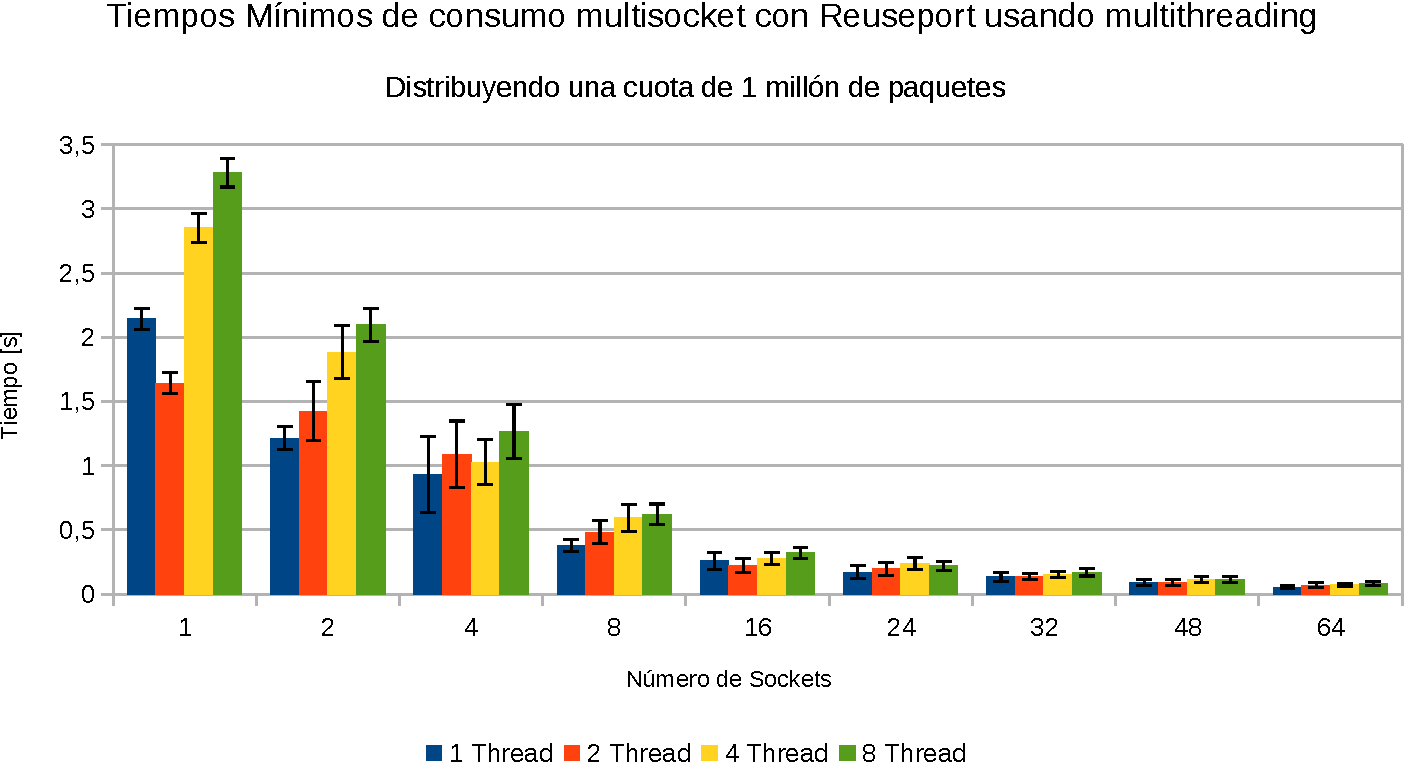
\includegraphics[width=.47\textwidth]{resultados/reuseport21-crop.pdf}
		\label{fig:reuseport2min}
	}\hfill
	\subfigure[]{
		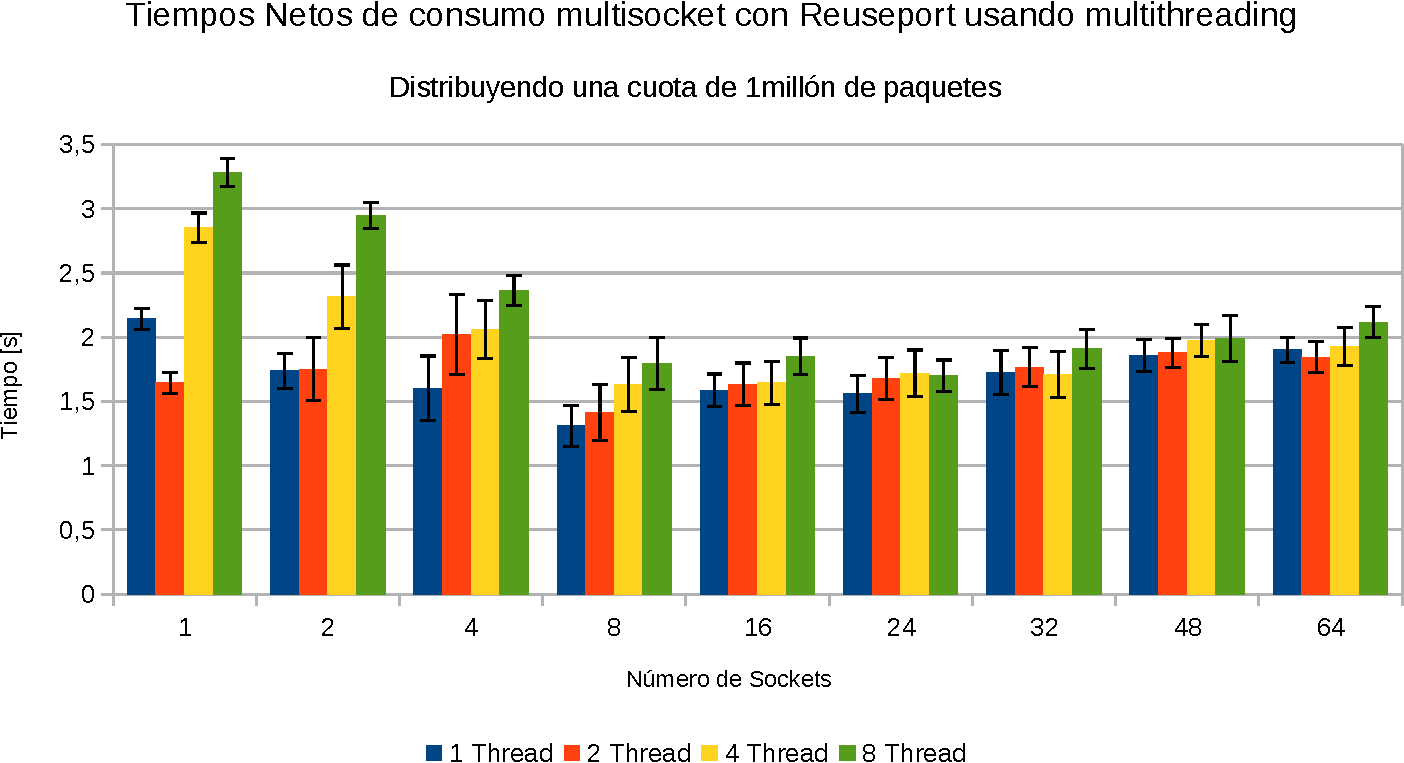
\includegraphics[width=.47\textwidth]{resultados/reuseport22-crop.pdf}
		\label{fig:reuseport2neto}
	}
	\caption{Graficos del resultado del nuevo caso de estudio incorporando lectura con múltiples hilos. En la leyenda de cada gráfico se indica el número de threads que consumen concurrentemente cada socket con reuseport.}
	\label{fig:resultadosReuseport2}
	\hspace*{\fill}
\end{figure}

Los resultados están ilustrados en el gráfico de la figura \ref{fig:resultadosReuseport2}. El primer gráfico que indica los tiempos mínimos \ref{fig:reuseport2min} evidencia que la incorporación de hilos para lectura concurrente mayoritariamente empeoró el desempeño registrado sin concurrencia, sin embargo, las tendencias se conservan a lo largo de la prueba, dando siempre tiempos mínimos mejores a medida que se emplean más sockets. De ésta forma, la clave en los tiempos mínimos parece ir más relacionada a la cantidad de sockets que se empleen en cada caso. En el segundo gráfico que ilustra los tiempos netos de la prueba \ref{fig:reuseport2neto} se identifica como la ejecución con threads perjudica siempre el desempeño de reuseport, degradando los tiempos y no brindando ninguna mejora práctica. Es interesante resaltar también que a partir de valores muy altos, parece ser despreciable el sobrecosto que añade tener más threads en cada socket, comportamiento que apoya el planteamiento inicial de que, a una menor cuota de consumo, el sobrecosto disminuye.

\subsection{Incorporación de Multithreading con Processor Affinity}
Similar al estudio del capítulo anterior en la arista de distribución de carga, en ésta sección se evaluó el desempeño de Reuseport en escenarios donde múltiples hilos de consumo acceden al socket, y fuesen distribuidos lógicamente entre los distintos CPU del sistema aprovechando la técnica de \emph{Processor Affinity}. En éste caso, se evaluaron 3 configuraciones:

\begin{description}
\item[SOsched] Los hilos son distribuidos por el mismo sistema operativo a través de la oepración de su algoritmo de schedulling. Es la base de comparación para con los demás esquemas de distribución.
\item[All0sched] Los distintos hilos de ejecución se alocan en el mismo core (core 0 por simplicidad). Persigue aprovechar localidad de datos en la ejecución simultanea de los hilos.
\item[Equitativesched] Los hilos se distribuyen equitativamente entre los cores lógicos del sistema, persiguiendo una distribución de carga entre unidades de procesamiento real.
\end{description}

\begin{figure}[h!]
	\centering
	\subfigure[]{
		\centering
		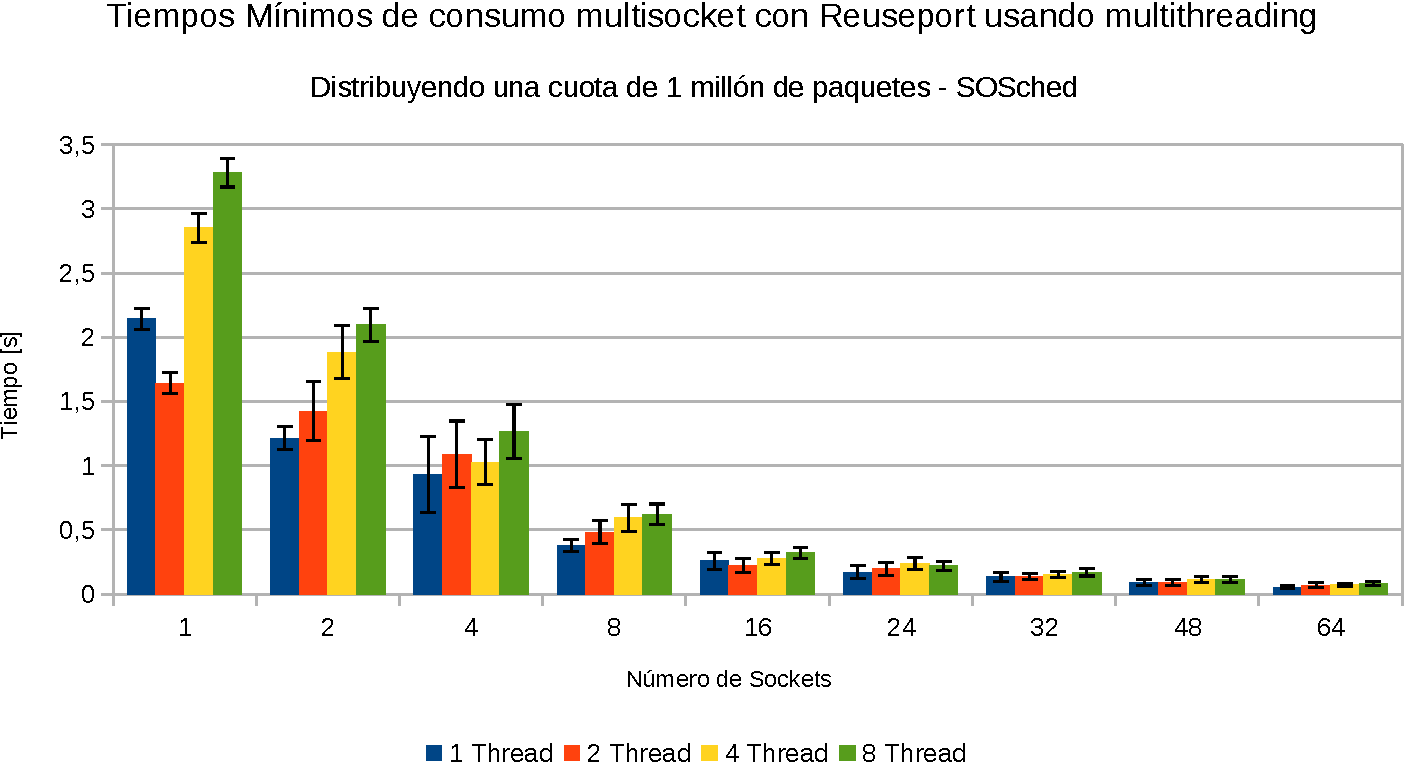
\includegraphics[width=.47\textwidth]{resultados/reuseport31-crop.pdf}
		\label{fig:reuseportsomin}
	}
	\subfigure[]{
		\centering
		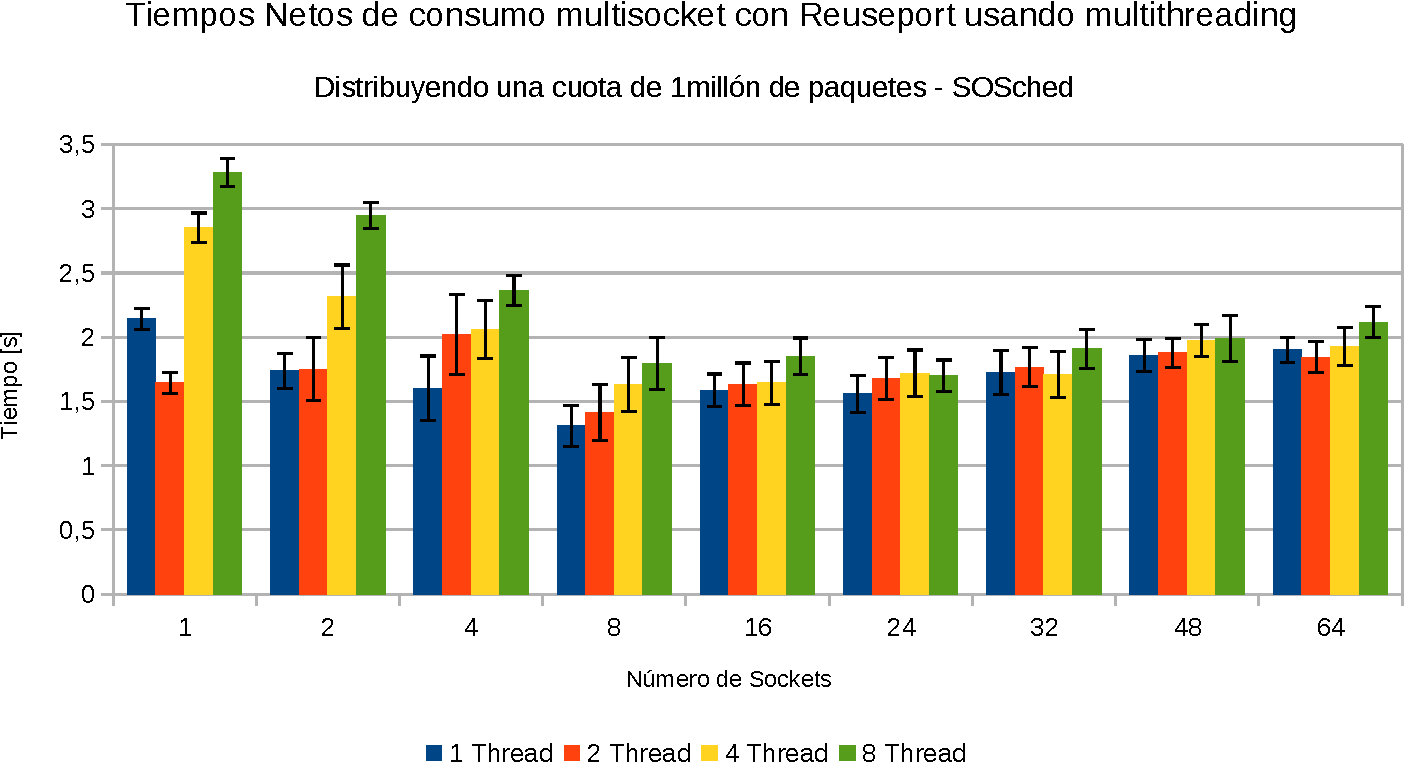
\includegraphics[width=.47\textwidth]{resultados/reuseport32-crop.pdf}
		\label{fig:reuseportsoneto}
	}
	\subfigure[]{
		\centering
		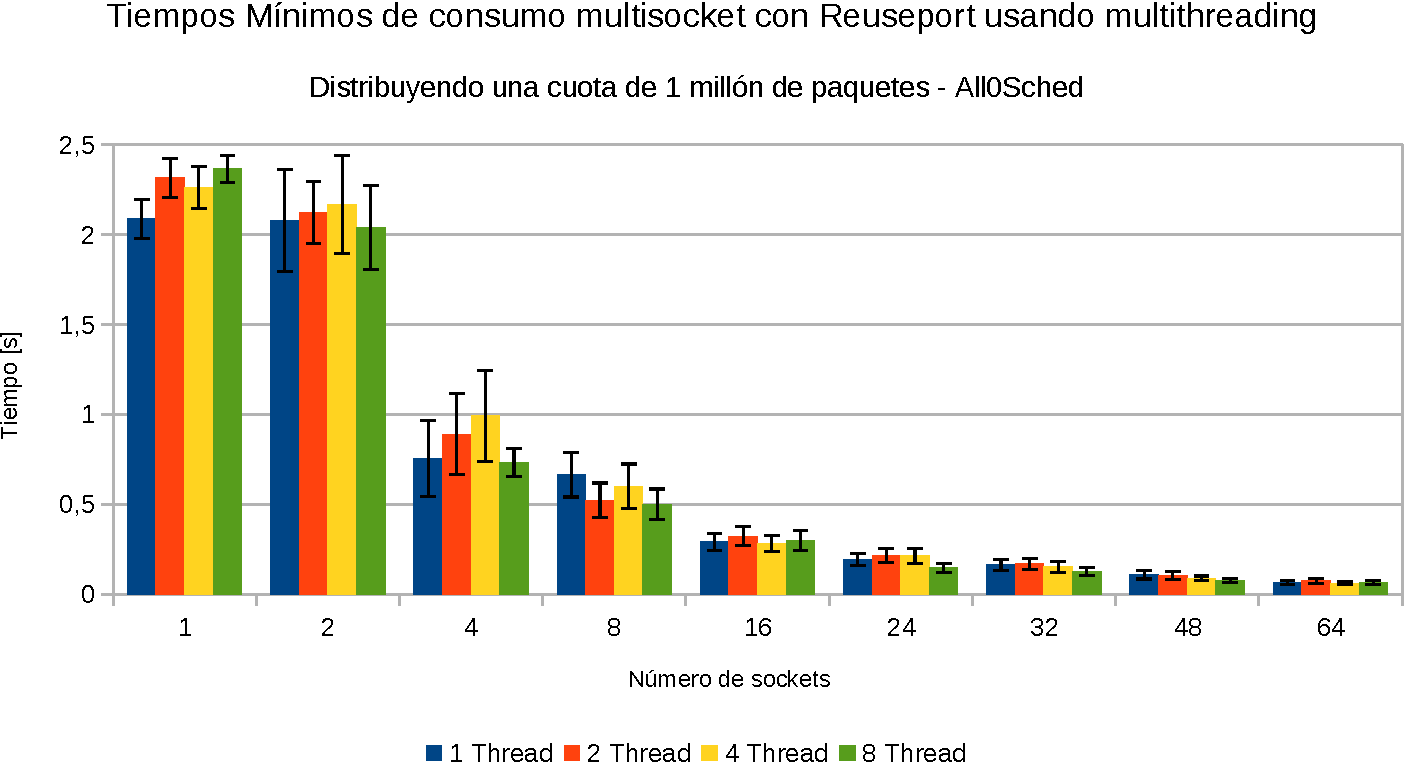
\includegraphics[width=.47\textwidth]{resultados/reuseport33-crop.pdf}
		\label{fig:reuseportall0min}
	}
	\subfigure[]{
		\centering
		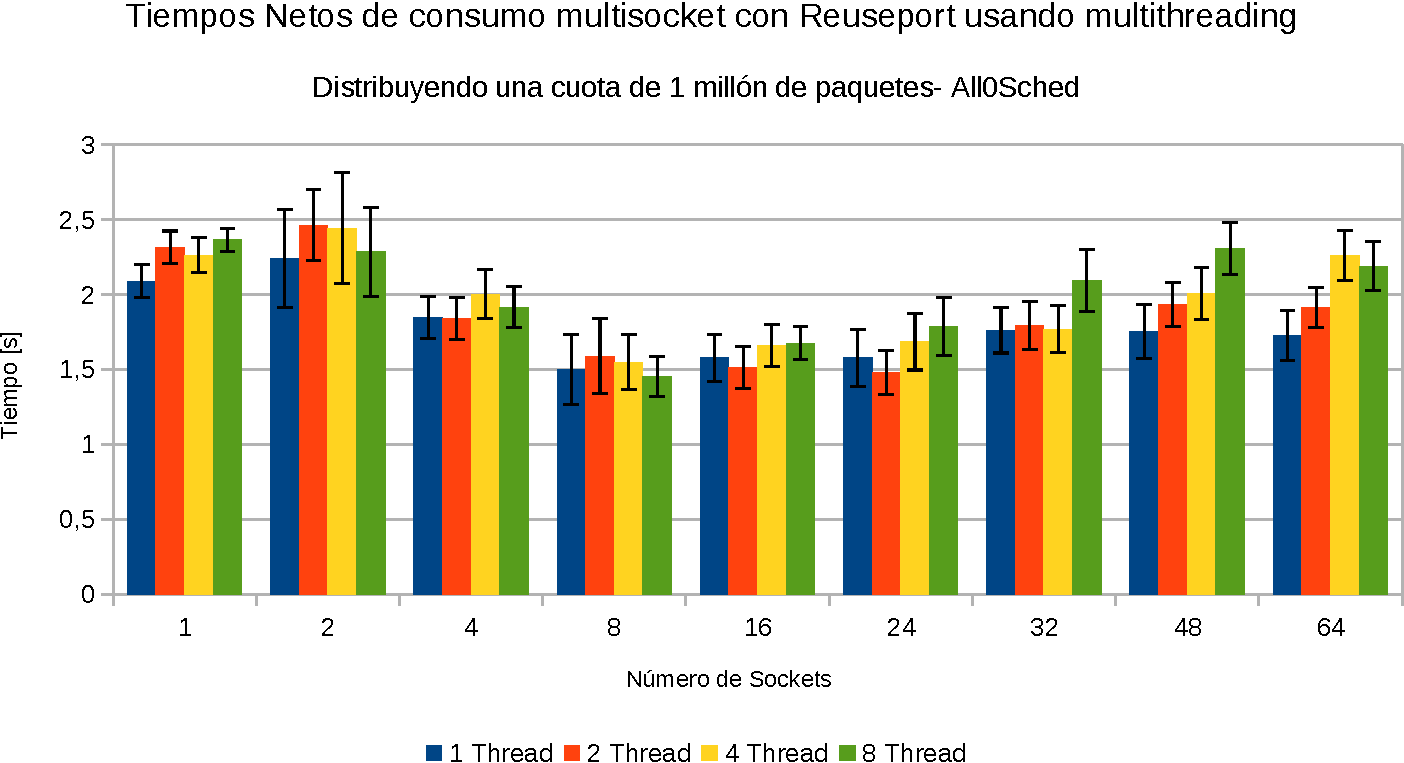
\includegraphics[width=.47\textwidth]{resultados/reuseport34-crop.pdf}
		\label{fig:reuseportall0neto}
	}
	\subfigure[]{
		\centering
		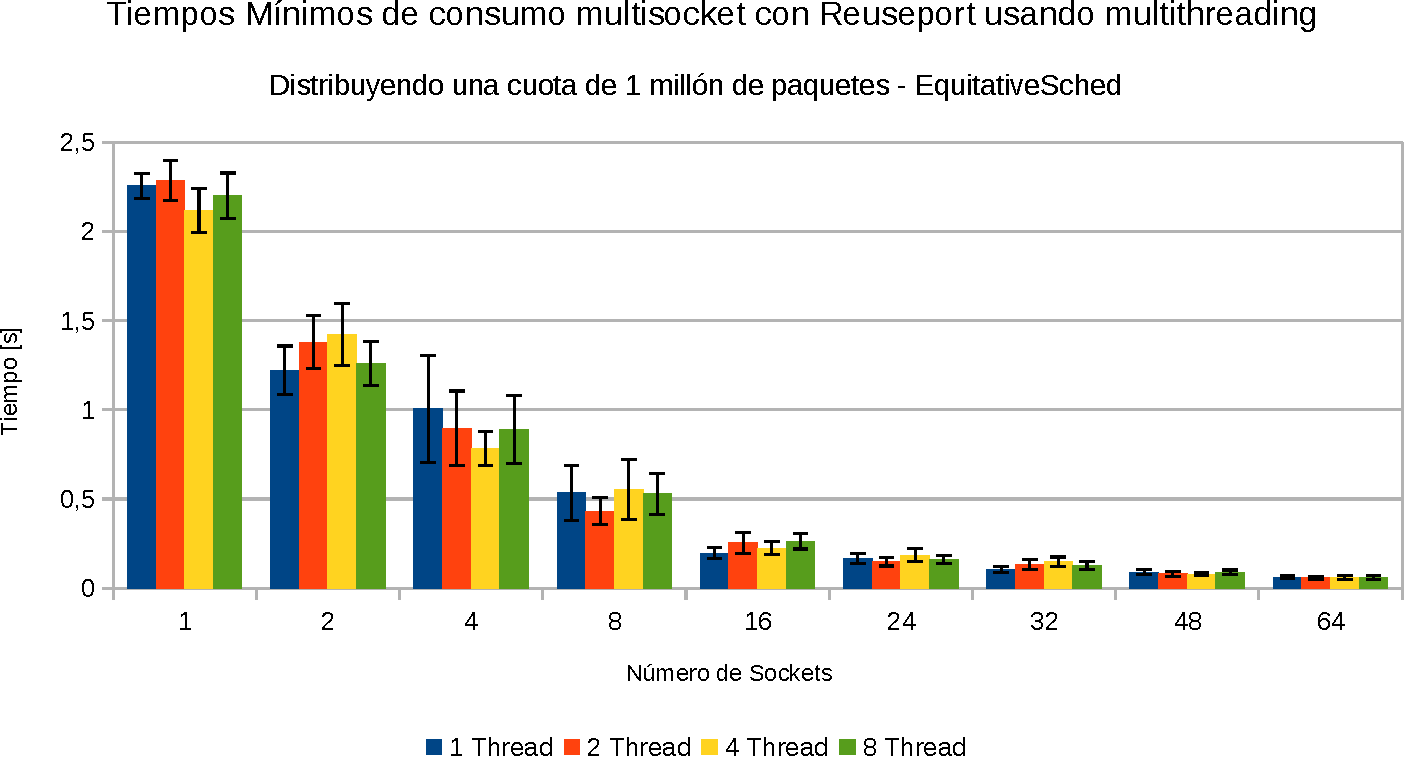
\includegraphics[width=.47\textwidth]{resultados/reuseport35-crop.pdf}
		\label{fig:reuseporteqmin}
	}
	\subfigure[]{
		\centering
		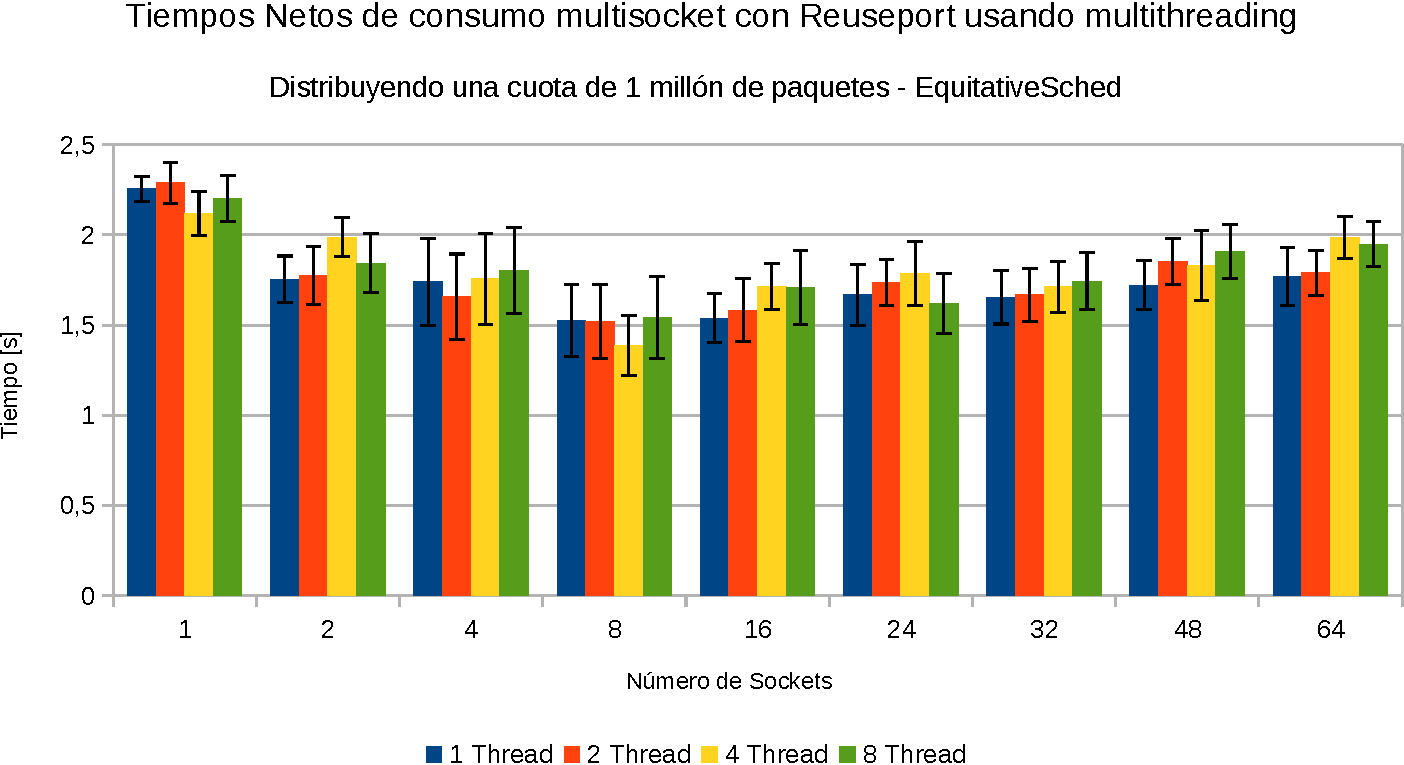
\includegraphics[width=.47\textwidth]{resultados/reuseport36-crop.pdf}
		\label{fig:reuseporteqneto}
	}
	\caption{Graficos de los resultados del nuevo caso de estudio incorporando lectura con múltiples hilos empleando distintas estratégias de \emph{processor affinity} en los hilos.}
	\label{fig:resultadosReuseport3}
\end{figure}

Los resultados de esta evaluación se encuentran en la figura \ref{fig:resultadosReuseport3}. La primera observación relevante a destacar es que, en general, las tendencias de comportamiento tanto en tiempos mínimos como en tiempos netos, se preserva independiente del mecanísmo de distribución de threads que se emplee. Los registros de tiempos mínimos mantienen su tendencia de decrecimiento a medida que se incorporan más sockets y la tendencia de los tiempos netos preserva su decaimento en torno a los 8 sockets, sin variaciones importantes entre esquemas.

Sin embargo, hay ciertos elementos a destacar que se evidencian en los nuevos esquemas de distribución. Tanto en la configuración \emph{Equitativesched} (Fig. \ref{fig:reuseporteqmin} y \ref{fig:reuseporteqneto}) como en \emph{All0sched} (Fig. \ref{fig:reuseportall0min} y \ref{fig:reuseportall0neto}) ocurre un fenómeno interesante en la disperción o variación de los valores al incorporar threads. En ambos esquemas las variaciones usando distinta cantidad de threads en configuraciones con bajo número de sockets se presenta un desempeño bastante parejo, a diferencia del esquema \emph{SOsched} (Fig. \ref{fig:reuseportsomin} y \ref{fig:reuseportsoneto}). Una tendencia que se mantiene al aumentar el número de sockets consumiendo datos haciendo las difernecias de tiempo muy pequeñas entre usar uno o muchos threads por socket. Éste comportamiento refleja que las técnicas de \emph{processor affinity} tienen buenos resultados en balancear la carga cuando se emplean pocos sockets y la cuota de consumo de cada uno es más alta, permitiendo un mejor balance de tiempos entre los threads que consumen cada socket, pero aún así no consiguen batir los tiempos obtenidos por reuseport. La razón de ello apunta a ser que, antes de incorporar paralelísmo usando hilos, se llega a un límite de rendimiento del socket mismo que no puede ser superado aplicando concurrencia de ésta manera, y que es precisamente el problema detectado en un principio.

\subsection{Análisis y Discusión de Resultados}
Como se aprecia de los resultados experimentales, la incorporación de multithreading en el consumo de datos desde una estructura socket con soporte para reuseport siempre degrada el rendimiento completo del caso de estudio, independiente de si se emplean esquemas de distribución de carga entre los núcleos de procesamiento efectivo. Resulta interesante que más allá de las estratégias que se adopten para la mejor distribución de carga, las variaciones no permiten justificar una verdadera ganancia o pérdida entre esquemas que se adopten, siendo simplemente sobrecargas con respecto al esquema de distribución propio del sistema oeprativo.

Éste resultado viene a confirmar la conclusión de los estudios del capítulo anterior que terminan por postular que es la misma estructura socket de Linux la que no cuenta con un diseño compatible con técnicas de consumo concurrente, degenerando siempre en escenarios de degradación de performance generalizada en su consumo.

\section{Aspectos Negativos}
El esquema que propone reuseport replantea uno de los principios fundamentales que postula el modelo OSI, que es la relación ''uno a uno'' entre estructuras sockets y direcciones de puertos locales. Como reuseport plantea la compartición de puertos locales se pierde la exclusividad de los mismos para cada socket. Otra caracteristica que trastoca ésta alternativa es la modificación en la manera de programación de aplicaciones. Como se mencionó, el uso de ésta técnica está condicionada a la habilitación de dicha opción a los sockets previo al momento de su acoplamiento con el puerto local a escuchar. Ésta situación significa en la práctica estar concientes de que toda aplicación que desee hacer uso de ésta característica debe modificar secciones profundas de su implementación en el código fuente para habilitarla, siempre y cuando el sistema donde se trabaje disponga de soporte para la misma.

Por otro lado, dado su funcionamiento la opción de reuseport está incorporada como código fuente del kernel de Linux, estando disponible según sus creadores en los kernels con versiones posteriores a la 3.9 (Finales del año 2013), ello no es del todo correcto. Un caso de ello son las distribuciones de Linux basadas en Debian --incluido el popular Ubuntu-- donde se han presentado varios problemas en versiones recientes las cuales, a pesar de contar con kernels 3.9+ y tener la implementación fuente de reuseport, poseen la constante de activación de la característica (el flag \verb=SO_REUSEPORT=) como código comentado y no utilizable\footnote{\url{https://lists.debian.org/debian-kernel/2015/02/msg00260.html}} u otros casos de distribuciones de linux que siguen la dinámica de actualización basadas en \emph{continuous release} que no incorporan los cambios encesarios para dar soporte a las funcionalidades de reuseport\footnote{\url{https://github.com/circus-tent/circus/issues/699}}, lo cual dificulta el uso de ésta opción al no dejarla disponible para el uso de los programadores de aplicaciones o llevando a errores de programas en el peor caso.

Una última dificultad asociada al uso de la opción reuseport se relaciona con su documentación. La documentación asociada a ésta característica es muy escasa, reducíendose prácticamente a la implementación misma disponible en el código fuente del propio kernel de Linux. No existe documentación a nivel de usuario que permita comprender ni mucho menos manipular las características de la opción en sí misma. En esa misma linea, aparece como un problema la implementación de ésta característica al ser una opción \emph{hardcodeada} en el kernel mismo de Linux, lo que hace inviable pensar cualquier modificación doméstica pensando en querer aprovechar su funcionamiento con ciertas modificaciones o adaptada a escenarios especiales. Ello pues toda modificación se traduce en modificar, recompilar e instalar todo un nuevo kernel, entendiendo en primer lugar lo complicado de dicha tarea, y en segunda instancia, sucitando el riesgo de posibles inestabilidades en el resultado, algo que en la práctica es inaceptable en entornos de producción. Ésto último da a entender que la característica reuseport no está pensada para ser modificable según escenarios especificos de operación.